\documentclass{article}
\usepackage{amssymb}
\usepackage{amsfonts}
\usepackage{amsmath}
\usepackage{amsthm}
\usepackage{url}
\usepackage{graphicx} 

%\usepackage[perpage,symbol*]{footmisc}

%\DefineFNsymbols*{daggers}{\dagger\ddagger{\dagger\suck\dagger}{\ddagger\ddagger}*{**}{***}}
%\setfnsymbol{daggers}


\begin{document}
\title{Internal $msms$ Manual} 
\maketitle 

\section{Introduction}   
 
$msms$ (ms mit\footnote{mit is ``with'' in German} selection) or $(ms)^2$ is a
program for simulation of different demographics and structured populations with
selection, using a forward-backward approach. Generally, it supports everything
that ms does, but with selection at one locus (\cite{ewing_2010}).
 
One goal of the project is to produce code that is modular and accessible for
extension by others. Currently, this means that the source and binary are always
distributed together to allow for critiquing, changes and patch submissions.

The purpose of this manual is not to provide a user guide, but to provide
details of the internals of the program. That is, to provide extra documentation
over and above the source code in a more generally accessible manner. 

\subsection{Simulation Outline}

The simulation uses a two-step method. First, we simulate forward in time,
keeping track of the frequency of the beneficial allele using a standard Wright 
Fisher model with demographic structure. This means that the number of
individuals in each successive generation is a binomial random variable with
a parameter dependent on the previous generation. The details are given below. 

Once the forward simulation is completed, we then use the coalescent to track
sampled individuals back in time, conditional on the frequency of the beneficial
allele determined from the forward simulation. This coalescent includes
migration, recombination and mutation of the beneficial allele. All parameters
can be functions of time, including demographic models and parameters. 

% The coalescent simulation is designed to be accurate within the normal coalescent
% approximation limits, even with quite extreme parameter choices. Furthermore,
% explicit events can be tracked on the tree if desired\footnote{this is not fully
% implemented yet}. For example, we may wish to track when recurrent mutations
% occur. We can specify this at simulation time and get some summary statistics or
% tree labels on the events. However, if we are not so interested in such things,
% we incur almost no overhead when not tracking different events.

\section{Forward Simulations}

\newcommand{\saa}{s^{aa}}
\newcommand{\saA}{s^{aA}}
\newcommand{\sAA}{s^{AA}}
\newcommand{\bs}[1]{\boldsymbol{#1}}

We consider a standard structured Fisher Wright population with two alleles $a$
and $A$ at a single locus. We assume that the allele $A$ is beneficial and that
we have a diploid population. The fitness values for the $i$th deme is
$1+\saa_i$, $1+\saA_i$, $1+\sAA_i$ for genotype $aa$, $aA$, and $AA$,
respectively. Migration  from deme $j$ to deme $i$, is defined as the proportion $m_{ij}$ of
deme $i$ that is made up of migrants from deme $j$. We let $m_{ii}=1-\sum_j
m_{ij}$, which is the proportion of nonmigrants in deme $i$.

Let $\bs{x}$ be a vector $(x_1,x_2,\ldots)$ where $x_i$ is the
relative frequency of the beneficial allele $A$. Therefore $x_i=n_i/(2N_i)$,
where $N_i$ is the population size of deme $i$, and $n_i$ is the number of $A$
copies in deme $i$.  

The life cycle is selection, mutation, migration, and random mating. The census
occurs with the formation of zygotes from the infinite gamete pool. Deviations
from HWE within each deme due to sampling are ignored. Selection occurs at the
zygotic stage and separately within demes. 

Now consider a single deme $i$ with proportion $x_i$ of the beneficial allele.
From HWE, the amount of beneficial alleles after selection but before migration
is,
\begin{align}
	\eta_{i}^A=x_i\left(1+(1-x_i)\saA+x_i\sAA\right)
\end{align}
and the amount of the nonbeneficial alleles is 
\begin{align}
	\eta_{i}^a=(1-x_i)\left(1+x_i\saA+(1-x_i)\saa\right). 
\end{align}
We use the term {\it amount} to indicate that these are not proportions, ie
are not normalized. Now if we consider the amount of beneficial alleles in deme $i$ that
comes from the migrants from deme $j$, we multiply the amount of
beneficial alleles after selection in deme $j$ by $m_{ij}$. If we consider all
demes, including the nonmigrants from the $m_{ii}$ term, the amount of
beneficial alleles and nonbeneficial alleles after selection and migration are, 
\begin{align}
	\eta^A_i&=\sum_j m_{ij} x_j \left(1+(1-x_j)\saA+x_j\sAA\right)
	\label{eq:selected}\\ 
	\eta^a_i&=\sum_j m_{ij}(1-x_j)\left(1+x_j\saA+(1-x_j)\saa\right)
	\label{eq:unselected}
\end{align}
and we have redefined both $\eta^A_i$ and $\eta^a_i$. 

We can now write the new frequency $x_i'$ in an infinite population by
normalizing as follows, 
\begin{align}
	x'_i=\frac{(1-\nu)\eta_i^A+\mu \eta_i^a}{\eta_i^A+ \eta_i^a}
	\label{normalized}
\end{align}  
where $\mu$ is the mutation rate from $A \to a$ and $\nu$ is the mutation rate  
from $a \to A$. 

We now sample the ``infinite'' population with a binomial random variable and
thereby include genetic drift. The number of $A$ copies in the next generation
$n_i'$ is given by
\begin{align}
	\Pr(n_i'|n_i)=\binom{2N_i}{n_i'} (x_i')^{n_i'}(1-x_i')^{2N_i-n_i'}.
	\label{eq:binom}
\end{align}
We then sample this using a modified library from the colt
project\footnote{\url{http://acs.lbl.gov/~hoschek/colt/}}. The simulation
proceeds until some stopping condition is met. 

% \subsubsection*{Haploid Populations}
% 
% \newcommand{\sa}{s^a}
% \newcommand{\sA}{s^A}
% 
% In the haploid case we only have two selection coefficients, $1+\sA$ and
% $1+\sa$. The formulas \ref{eq:selected} and \ref{eq:unselected} simplify to
% \begin{align}
% 	\eta_i^A&=\sum_j m_{ij} x_j (1+\sA) \\
% 	\eta_i^a&=\sum_j m_{ij} (1-x_j)(1+\sa).
% \end{align} 
% Equation \ref{normalized} stays unchanged while equation \ref{eq:binom} is
% changed to,
% \begin{align}
% 	\Pr(n_i'|n_i)=\binom{N_i}{n_i'} (x_i')^{n_i'}(1-x_i')^{N_i-n_i'}.
% \end{align}

\section{Coalescent Simulations}

Coalescent simulations are somewhat more involved due to recombination and
selection. The coalescent rate is dependent on population size. However, the
individuals that have the beneficial allele cannot coalesce with individuals that
don't have the allele. Thus, the ``virtual population size'' for a lineage in
say, the selected class, is a function of time. Further, it is not a
well-behaved function of time since we include drift. This complication extends
to most events. The events considered are migration, coalescence, recombination,
and mutation at the selected locus.

The simplest method is to use a generation by generation method. That is, we
check in each generation if an event occurs with a probability that produces the
correct geometric distribution where we define these probabilities later. This is
the method used by Yuseob Kim's selective sweep program, with interval rescaling
to ensure that all events are sufficiently rare. However, we use an explicit $N$
because of selection (i.e. we don't ``scale'' parameters, and $N=10^6$ will mean
that on the order of $10^6$ tests need to be done), and the complexity scales
with $N$, whereas with the standard coalescent it scales with sample size which
is much smaller than $N$.  Since this method is quite slow, regardless of the
rescaling used, we have implemented a faster method that is outlined below.


\subsection{Implementation Outline}

When we are not in a selection phase, normal coalescent simulations are
performed. That is, an exponential random variable is produced for a small set
of events, then the shortest exponential variable is taken, and finally, the
details of the event are decided; which often requires more random numbers to
choose the specific event. This is reasonably well-established in the
literature and is what $ms$ also does.

When we are in a selection phase, we first generate exponential random variables
for recombination, the only event that is independent of allele frequencies, and
take the first event. We then generate more exponential variables, using the fast
coalescent method (described below) with the shortest current exponential time
as a parameter. This way the fast simulations can return faster in many cases. Finally, we pick the
event with the shortest time and ``complete'' it as above.

It should be noted that for most events we must generate  independent event
times for each deme and each allelic class due to the dependence on the allele
frequencies. For example, we must generate a coalescent event time for each deme
and each class, and pick the smallest result because the allele frequencies in
each deme vary stochastically.

\subsection{Fast Coalescent Simulations}

The discrete method above produces geometric waiting times between events. We can
approximate this with an exponential, with reasonably good accuracy; this is in
fact what the original Kingman Coalescent does. So rather than just checking the
probability of an event at generation $t$, we can produce an exponential random
variable instead. However, we need to be able to take into account the changing
rate of the process. Without considering a specific event, we just discuss the
generic scheme used in the code. 

\renewcommand{\d}{\textrm{d}}

For concreteness and simplicity, we assume that we have a constant rate $\lambda$
over a time interval $\d \tau$. The cumulative probability function of the
exponential distribution is
\begin{align}
	\Pr (X \leq \tau)=1-e^{-\lambda \tau}.
\end{align}
So the probability of an event not happening in an interval of length $\d \tau$
is just the complement
\begin{align}
	\Pr (\d \tau < X) = e^{-\lambda \d \tau}.
\end{align}
Let $\lambda_t$ be the rate as a function of generations with $t \in
\mathbb{N}$ and $t= \lfloor \frac{\tau}{\d \tau} \rfloor$. We assume that there
is a constant part, and a variable part. So $\lambda_t = \lambda \alpha_t$ and
$\alpha_t$ is now the function of generations and $\alpha_t>0, \forall t$ . The
probability that an event does not happen after $n$ generations is 
\begin{align}
	\Pr (n<N) &= \prod_t^n e^{-\lambda \alpha_t \d \tau} \\
	&= e^{-\lambda \d \tau \sum_t^n \alpha_t}.
	\label{math:cumulant}
\end{align}
This result can be used to generate exponentially distributed time
intervals efficiently as follows. Let $U$ be a uniform random variable on the
interval $(0,1]$. We can equate
(\ref{math:cumulant}) with U and solve for $n$. We further simplify by setting
$\d \tau=1$ as $\tau$ is in generations. We have
\begin{align}
	U&=e^{-\lambda \sum_t^n \alpha_t} \\
	\ln U&=-\lambda \sum_t^n \alpha_t \\
	\frac{-\ln U}{\lambda}&=\sum_t^n \alpha_t .
	\label{math:rand}
\end{align}
We can then sum from the initial generation until the right hand side of
(\ref{math:rand}) is larger than the the left hand side and get a discrete
estimate of an exponential variable\footnote{i.e. this is in fact a geometric
distribution. However, this is only an intermediate step}. 

Because we are generating many such time intervals, and because we only choose
the shortest interval, we can futher optimise this process by only summing up to
the smallest $n$ we have observed so far. If the right hand side of equation
(\ref{math:rand}) is still larger than the left hand side, we know that the new
event cannot have a smaller time interval than the current $n$. If however the
summation does excede the left hand side, the event type and $n$ is updated
with the new values. 

We futher extend this to include fractional generations. Let $\tau_0$ denote
the current real valued time and we wish to determine the time of the next event
$\tau_n$. The initial generation for the sum is $t_0=\lfloor \tau_0 \rfloor$.
First, we find largest integer $n$ such that 
\begin{align}
	\frac{-\ln U}{\lambda} \geq \alpha_{t_0}(\lceil \tau_0 \rceil
	-\tau_0)+\sum_{t=t_0+1}^{n} \alpha_t
\end{align}
holds. Let $\tau_n=\tau_0+n-t_0+\delta$ and 
\begin{align}
	\delta \alpha_{n+1}=\frac{-\ln U}{\lambda}-\alpha_{t_0}(\lceil \tau_0
	\rceil -\tau_0)+\sum_{t=t_0+1}^{n} \alpha_t.
\end{align}
In words, we have used the rectangle rule to ``integrate'' the discrete values
of $\alpha_t$ over continuous time. This has the property that if
$\alpha_t$ is a constant, then we recover true exponential waiting times as per
the nonselected case. This also permits that events can happen with time
intervals smaller than one generation. This can be important when one is
studying the limits of strong selection for example.   


\subsection{Coalescent Events}

Coalescent events can only happen between lineages in the same class and the
same deme. Thus, there is a dependence on frequency of the selected allele as
stated earlier.  

Let $k_i^A$ be the number of lineages in deme $i$ that is in the
selected allelic class, ie with allele $A$. The coalescent rate between these
lineages is 
\begin{align}
	R_c^A=\frac{k_i^A(k_i^A-1)}{4N_i x_i}
\end{align} 
or
\begin{align}
	R_c^a=\frac{k_i^a(k_i^a-1)}{4N_i (1-x_i)}
\end{align}
for the unselected allelic class. Thus, when using the fast coalescent method,
we set  $\alpha_t=\frac{1}{x_i(t)}$ or $\alpha_t=\frac{1}{1-x_i(t)}$ as
appropriate.
 
\subsection{Migration} 

Migration when there is no selection is simple because the definition of $m_{ij}$
is constructed to make it simple. Recall that $m_{ij}$ is defined as the
proportion of deme $j$ that is made up of migrants from deme $i$. If we trace a
lineage back in time, the probability that it migrates from deme $j$ to deme $i$
backwards in time is just $m_{ij}$. However, we need to consider the different
allelic classes. That is, if a lineage migrates between demes, it cannot change
allelic classes.

The total proportion of deme $j$ that is in the selected allelic class is just
$x_j$. While the total proportion that migrated from deme $i$ is $m_{ij}$, and
so the total proportion of migrated individuals that are in the selected allelic
class is $\frac{x_i m_{ij}}{x_j}$. Hence, the migration rate from deme $i$ to
$j$ in forward time\footnote{Thus, in backward time the lineages move from
deme $j$ to deme $i$.} is
\begin{align}
	R_m^A&=k_j^A \frac{x_i m_{ij}}{x_j} \\
	R_m^a&=k_j^a \frac{(1-x_i) m_{ij}}{1-x_j}.
\end{align}
Again, we can now set $\alpha_t=\frac{x_i(t)}{x_j(t)}$ or
$\alpha_t=\frac{1-x_i(t)}{1-x_j(t)}$, respectively, for the selected class or
unselected class. 

\subsection{Mutation at the Selected Locus}

Mutation at the locus under selection also gains a dependence on the proportions
of selected to unselected classes. We only consider recurrent mutation from the
wild type to the selected allele in forward time. That is, in backwards time a
lineage can only move from the selected class to the unselected class.

Consider the proportion of the selected alleles in a deme that arises from
mutation on the selected locus. This is simply $\mu(1-x_i)/x_i$, that is the
total amount of selected alleles that arise from mutation $\mu (1-x_i)$
normalized by the total amount of selected alleles. So the rate backwards in
time is 
\begin{align}
	R_\mu=\frac{\mu (1-x_i)}{x_i}. 
\end{align}
Thus $\alpha_t=(1-x_i(t))/x_i(t)$

A similar argument can be made for recurrent mutation in the opposite direction
and we arrive at $\alpha_t=x_i(t)/(1-x_i(t))$.

\subsection{Recombination}

The recombination rate is not directly affected by the allele frequencies.
However, there are a number of other considerations that make recombination the
most difficult event to implement.

First, we must consider the sequence model. We use an abstract continuous model
without considering an explicit mutation model at this stage. Here we only need
to consider which sections of a sequence are {\it active}, in that we can
observe the mutation process on that region from our sampled individuals. The
sequence here is just a set of nonoverlapping intervals that denote these active regions.
Furthermore, the regions are not constrained to have a summed length of 1, but
can be smaller or larger. We define a single active interval at sampling time as
$(0,1)$. Multiple loci can be easily added by simply defining more than one
active interval at sampling time.

\begin{figure}[hbtp]
\begin{center}
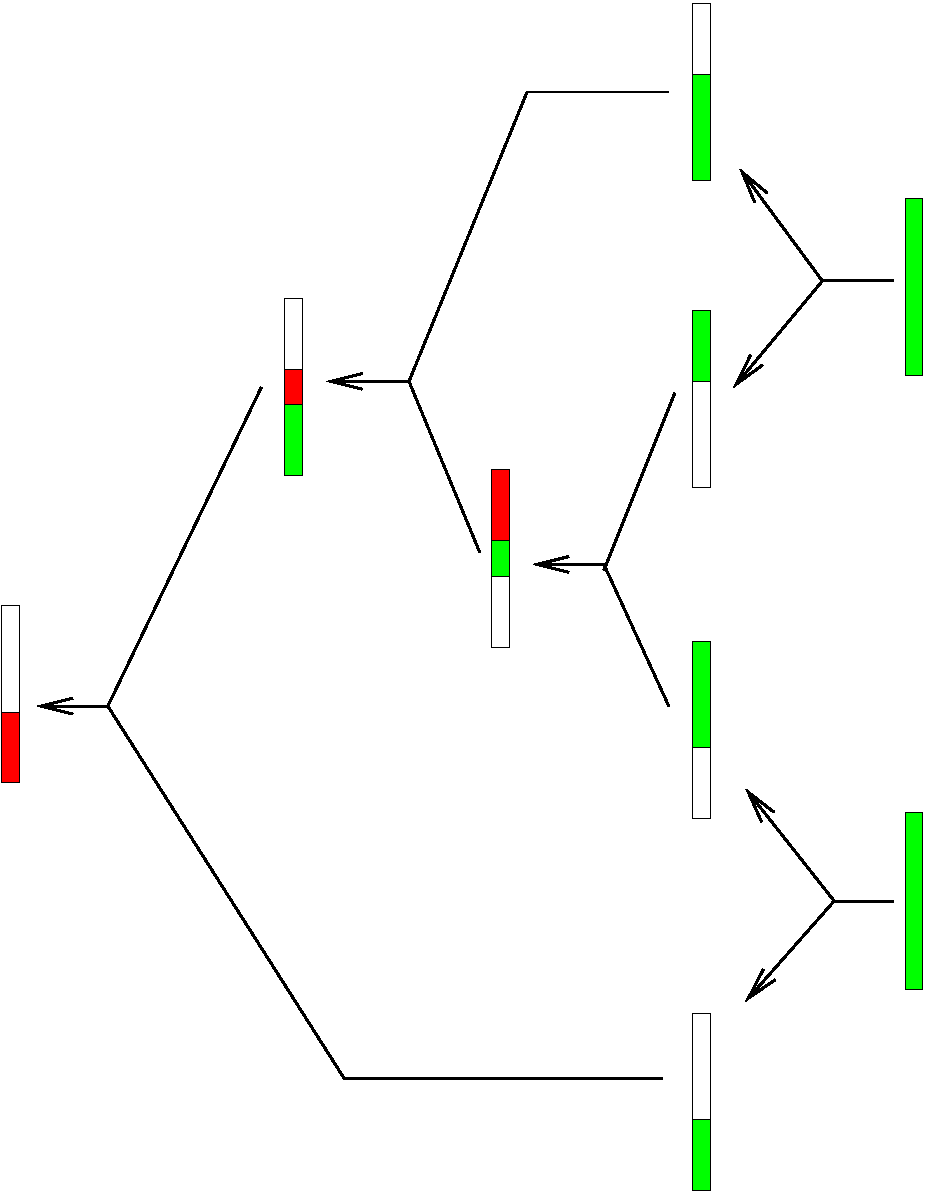
\includegraphics[width=0.5\textwidth,angle=-90]{recombination}
\end{center}
\caption[Recombination/Coalescent Example]{The figure shows how active regions
(green) change with recombination events and coalescent events. Recombination
events split active regions whereas coalescent events join them. However, some
regions may ``coalesce'' (red). In this case, the region is active below the
coalescent event but not active above the coalescent event.}
\label{fig:recomb}
\end{figure}

Ignoring selection, we consider a simple coalescent recombination graph in
figure \ref{fig:recomb}. Here just two sequences have recombination
events, and then the resultant 4 lineages coalesce. Going back in time, the
recombination events increase the number of lineages present by splitting the
active regions into complementary active regions. 

When we have a coalescent event, we use a union of the active region of both
coalescing lineages. However, we need to also consider {\it coalesced regions}.
That is, active regions that are no longer present in any other lineage. Such
regions are shown in red in Figure \ref{fig:recomb}, and are not active above a
coalescent event. But, they are active below the coalescent event. In other
words, we cannot observe a segregating site in our samples over the coalesced
region from a mutation that occurs above\footnote{Above here means further into
the past.} the coalescent event.

Over time, the total length of active regions reduces to zero, and we do not
need to run the coalescent simulation to the ultimate common ancestor of the samples.
Further optimization is needed when high recombination rates are used. It
is a fact that some recombination events result in unobservable lineages.
That is, a lineage with no active regions. This can happen if the cut site of a
recombination event happens outside the upper or lower bounds of the active
regions. Therefore, instead of using the recombination rate, we use the
observable recombination rate for each lineage. This is the distance between
the upper and lower bounds of active regions, times the recombination rate.

We note that at this stage we do not consider mutations above {\it coalesced
regions}, and thus we are in fact considering polymorphisms.


\subsubsection{Recombination with Selection}

When considering recombination with selection, we must take into account that
there is a selected locus somewhere on the sequence. The allele at this locus can
be either the selected allele, or the unselected allele. We do not explicitly tag
sequences with the allele but rather track lineages as either in the  selected
class or unselected class. The locus has a position on the sequence, and can be
some distance away from any active region. This has an impact on the observable
recombination rate because recombination between this selected locus and active
regions is observable. In other words, it changes the coalescent process.

When going forward in time, two different lineages are crossed over to form a
new lineage. Here are the  possibilities:
\begin{itemize}
  \item Both lineages are from the selected class, and the resultant
  recombinant is also in the selected class.
  \item Both lineages are from the unselected class, and the resultant
  recombinant is also in the unselected class.
  \item One lineage is from the selected class and one from the unselected
  class. The resultant recombinant can be either in the selected or unselected
  class. 
\end{itemize}
When moving backward in time during the coalescent phase, we start with the
resultant recombinant. Let $x$ be the relative frequency of the beneficial
allele at the time of recombination in a single deme. We have only two 
cases to consider. If the recombinant is in the unselected class, then at least
one source lineage is also in the unselected class. The second source lineage
for a recombinant is from the selected class with probability $x$. Otherwise, it
is from the unselected class. 

The complementary statement is true when the recombinant is from the selected
class. At least one source lineage must be from the selected class. The second
source lineage is from the selected class with probability $x$, and is from the
unselected class otherwise. 

Note that when the source lineages are from both classes, which lineage gets
what active region is defined by the recombination cut site. That is, if the
selected locus is on the left of the cut site and is selected, then the
``left'' lineage source must be from the selected class. 

Finally, we consider a simple case that one of the source lineages has no active
regions. This can be quite common when the selected locus is a long way from the
sequence locus. A recombination event can be swapped for a simple change in class
and hence, does not require an extra lineage to be tracked. That is, when
going back in time a selected class lineage may move into an unselected class,
as far as all active regions are concerned, or vice versa.

\section{Random Numbers}

The random number generator is not a default java random number generator, as
this has a period of only $2^{48}$ and fails some random number tests in the die
harder battery of random number tests. We have a fast random number generator
that passes all die harder tests and avoids the hyperplanes
problem\footnote{George Marsaglia, Random Numbers fall mainly in the planes,
PANS 1968,61(1)}, and has a period of $2^{128}-1$. The internal state 64 bit variable
that is incremented in a  m-sequence implemented via the {\it shift xor} method,
combined with a 64 bit Weyl sequence. Intermediate output is via the addition of
both sequences and masking. This is much faster\footnote{about 10 times faster in
fact} than Mersenne Twister, while still avoiding the LCG problems.

Note that other random number generators will be available in the future. Adding
a new random number generator has been designed to be as easy as possible. Note
that for some parameter choices, up to 50\% of the CPU time is spent generating
random numbers. 

\section{Current Status}

At the time of writing, $msms$ is almost a version 1. Currently, the version is
a release candidate, and we will pass the version 1 milestone once the first
round of bug reports and requests for enhancements has been considered.

Everything in ms is supported with the exception of gene conversion. 

% \subsection{Unit Tests}
% 
% Currently, there are no unit tests in the source. They were cleared out when
% re-factoring because they were bigger than the base code, and contained some
% bugs. New unit tests will be added but will only test a limited set of  sub
% components to avoid unneeded complexity.

% \subsubsection{Correctness}
% 
% The current code has been tested against Yuseob Kim's selective sweep program
% and against Hudson's MS program. However, using both migration and selection has
% not been directly compared to other programs as of yet. So testing with forward
% simulation programs will be undertaken shortly. Also, the tests have been
% done in an ad hoc manner. Full testing scripts will be added shortly. 
 

\subsection{Road Map}

Other than bug fixes, no major changes to the code are expected to be needed.
Some work on the code comments and extra developer documents will be
forthcoming. 

In the near future, we will add multiple selected alleles. This may require some
bigger changes. However, every endeavor will be made to avoid excessive
refactoring and to maintain compatibility with any 3rd party tools and
extensions. 

\section{Contributing}

Contact Greg Ewing (gregory.ewing@unive.ac.at) directly for details.
Currently, the source control is via {\tt git} and so patch submission is
probably the simplest way at this stage.


\bibliographystyle{natbib} 
\bibliography{Bio} 


\end{document}
